\subsection{Project Charter}
The project charter was generated at the end of the first sprint cycle. It will serve the purpose of maintaining a high-level understanding of project procedures, maintenance, and polices. The content will be generated from the latex format provided by Professor McMurrough. It will be stored as a forked GitHub Repository. It will be updated every sprint (if necessary), by committing changes to the aforementioned repository.

\subsection{Product Backlog}
The product backlog provides a list of high-level tasks that must be completed during sprints. The content will take the form of a table included in the presentation at the end of each sprint. It will be stored as a Google Document that all team members will have access to. It will be updated by changing the Google Document during sprints, with approval from all team members. 

\subsection{Sprint Planning}
Sprints shall be planned at the beginning of each sprint cycle via a scrum meeting of all team members. A Google Document will be created that assigns all team members their respective sprint goals and backlog items. This document will be stored on Google Documents and updated at the discretion of team members. Any member may edit this document, but only upon group consensus of the changes.

\subsubsection{Sprint Goal}
Every sprint shall have a sprint goal agreed upon by all team members at the first scrum meeting of a given sprint. This goal will be stored in the same document as the Sprint Plan, and updated at the discretion of the team members. Any member may edit this document, but only upon group consensus of the changes.

\subsubsection{Sprint Backlog}
Each sprint shall have a sprint backlog, which shall consist of a subset of the product backlog items. This document will consist of a table with story points attached to each task and will be stored in the same document as the sprint plan and goal. Changes to this backlog can only be made with approval from all team members.

\subsubsection{Task Breakdown}
During the first scrum meeting of each sprint, the product backlog will be broken down into individual tasks that shall be assigned to each team member during the creation of the sprint backlog. Each breakdown shall be agreed upon by all members, and assignments will be voluntary. The task breakdown can be changed with approval from all members. Until this occurs however, all team members are expected to work on their respective tasks, even if the breakdown is pending change. All members shall be repsonsible for logging the hours they spent on each task.

\subsection{Sprint Burndown Charts}
Upon completion of a sprint, a chart will be created and added to the sprint planning document which shows the total man-hours spent on each task as data points over time. This chart will also be included in the sprint overview presentation.

\begin{figure}[h!]
    \centering
    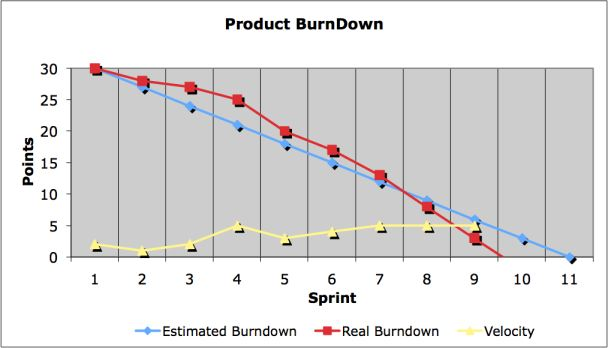
\includegraphics[width=0.5\textwidth]{images/burndown.jpg}
    \caption{Example sprint burndown chart}
\end{figure}

\subsection{Sprint Retrospective}
Upon completion of a sprint, a scrum meeting shall take place for which all team members must be present. This meeting's purpose shall be to determine what goals are being most effectively accomplished and which ones need resources reallocated, or labor redistributed.

\subsection{Individual Status Reports}
During each sprint, each team member will be responsible for logging their individual amounts of work performed for each task in the individual status report. These cannot be changed by any team member other than the one whose name appears at the top. These reports will be presented at the Spring Retrospective. They cannot be changed after this presentation.

\subsection{Engineering Notebooks}
Lorem ipsum dolor sit amet, quidam omnesque ea vis. Eum an aliquip legendos recusabo. Mea ex purto natum, ne movet fuisset sit. Labore audiam eos ad, facer ornatus posidonium ne ius, et eos duis delenit nusquam.

\subsection{Closeout Materials}
Lorem ipsum dolor sit amet, quidam omnesque ea vis. Eum an aliquip legendos recusabo. Mea ex purto natum, ne movet fuisset sit. Labore audiam eos ad, facer ornatus posidonium ne ius, et eos duis delenit nusquam.

\subsubsection{System Prototype}
Lorem ipsum dolor sit amet, quidam omnesque ea vis. Eum an aliquip legendos recusabo. Mea ex purto natum, ne movet fuisset sit. Labore audiam eos ad, facer ornatus posidonium ne ius, et eos duis delenit nusquam.

\subsubsection{Project Poster}
Lorem ipsum dolor sit amet, quidam omnesque ea vis. Eum an aliquip legendos recusabo. Mea ex purto natum, ne movet fuisset sit. Labore audiam eos ad, facer ornatus posidonium ne ius, et eos duis delenit nusquam.

\subsubsection{Web Page}
Lorem ipsum dolor sit amet, quidam omnesque ea vis. Eum an aliquip legendos recusabo. Mea ex purto natum, ne movet fuisset sit. Labore audiam eos ad, facer ornatus posidonium ne ius, et eos duis delenit nusquam.

\subsubsection{Demo Video}
Lorem ipsum dolor sit amet, quidam omnesque ea vis. Eum an aliquip legendos recusabo. Mea ex purto natum, ne movet fuisset sit. Labore audiam eos ad, facer ornatus posidonium ne ius, et eos duis delenit nusquam.

\subsubsection{Source Code}
Lorem ipsum dolor sit amet, quidam omnesque ea vis. Eum an aliquip legendos recusabo. Mea ex purto natum, ne movet fuisset sit. Labore audiam eos ad, facer ornatus posidonium ne ius, et eos duis delenit nusquam.

\subsubsection{Source Code Documentation}
Lorem ipsum dolor sit amet, quidam omnesque ea vis. Eum an aliquip legendos recusabo. Mea ex purto natum, ne movet fuisset sit. Labore audiam eos ad, facer ornatus posidonium ne ius, et eos duis delenit nusquam.

\subsubsection{Hardware Schematics}
\begin{figure}[h!]
    \centering
    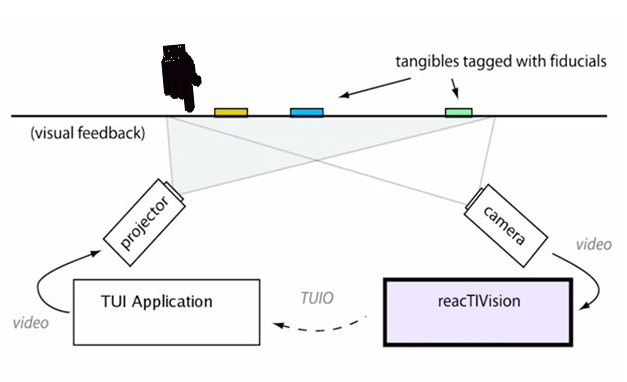
\includegraphics[width=0.5\textwidth]{images/Diagram.jpg}
    \caption{Example sprint burndown chart}
\end{figure}
A camera provides a real time video stream to reacTIVision. Then the source images have been encoded into the fiducial symbol with an unique ID number. TUIO is a communication protocol of reacTIVision that was designed to encode and transmit the attributes of tangible objects on a table's surface. In order to provide fast and reliable communication with local and remote client applications, TUIO defines a set of OSC (Open Sound Control) messages. These messages encode the fiducials' position, presence and transmit this data to the client applications. On the client side, these messages are decoded to add, update or remove events corresponding to the physical actions that have been applied to each fiducial marker.

\subsubsection{CAD files}
Lorem ipsum dolor sit amet, quidam omnesque ea vis. Eum an aliquip legendos recusabo. Mea ex purto natum, ne movet fuisset sit. Labore audiam eos ad, facer ornatus posidonium ne ius, et eos duis delenit nusquam.

\subsubsection{Installation Scripts}
\subsubsection{Hardware Installation}
A camera and a projector with wide angle lenses need to be placed underneath the table, so they can both cover the entire surface. The table's surface should be transparent, such as sanded glass with a blurring coating. To achieve a blurring surface, we need to place a sheet of ordinary tracing paper on the table. Also we should have a matte finish on the lower side of surface to avoid direct reflections of the projector lamp. 

\subsubsection{User Manual}
Lorem ipsum dolor sit amet, quidam omnesque ea vis. Eum an aliquip legendos recusabo. Mea ex purto natum, ne movet fuisset sit. Labore audiam eos ad, facer ornatus posidonium ne ius, et eos duis delenit nusquam.
